\chapter{View Incremental Decremental Multi-view Discriminant Analysis}
\label{ch:VIDMvDA}
\noindent {\textbf{\huge W}}e present in this chapter View Incremental Decremental Multi-view Discriminant Analysis (VIDMvDA), which is a classification method for 2D multi-view data. The motivation behind this method is similar to that of the other incremental methods presented in this thesis. However, those methods aimed to facilitate the addition/deletion of data samples, whereas VIDMvDA aims at supporting the addition/deletion of views. VIDMvDA is based on discriminant analysis and aims to reduce computational costs. It supports the addition or deletion of multiple views without retraining the model from scratch. All the updates in the model are obtained in a closed-form.

We present the formulations of VIDMvDA, experimental setup, and results in subsequent sections. We compare the proposed method with its batch counterpart (MvDA) on parameters such as- similarity of the discriminant subspace, classification accuracy, training time, and memory requirements. We also show that the sequence of addition or removal of views of data does not alter the final common discriminant subspace. We conclude this chapter by summarizing the features of VIDMvDA.






\section{Methodology}
\label{sec:VIDMvDA_Algo}
As we saw in section \ref{ssubs:Lit_MvDA}, the scatter matrices are made up of view-wise submatrices. These submatrices are computed in a pairwise manner from all the views. To add a new view, we must compute the scatter of this view with respect to each of the existing views and itself. For example, when the within-class scatter of the data samples belonging to $(v+1)^{th}$ view is to be updated, $\textbf{S}_{j(v+1)}$ and $\textbf{S}_{(v+1)j}$ for all \{$j = 1, \cdots, (v+1)$\} are computed. These pairwise submatrices are then appended onto the existing scatter matrix $\textbf{S}$. We also need to update the existing submatrices as the number of data samples per class used to compute the scatters changes after each increment. In the case of decrement, we delete the submatrices of the deleted view/s and update the remaining submatrices using the updated number of data samples per class.

\begin{figure*}[t]
	\centering
	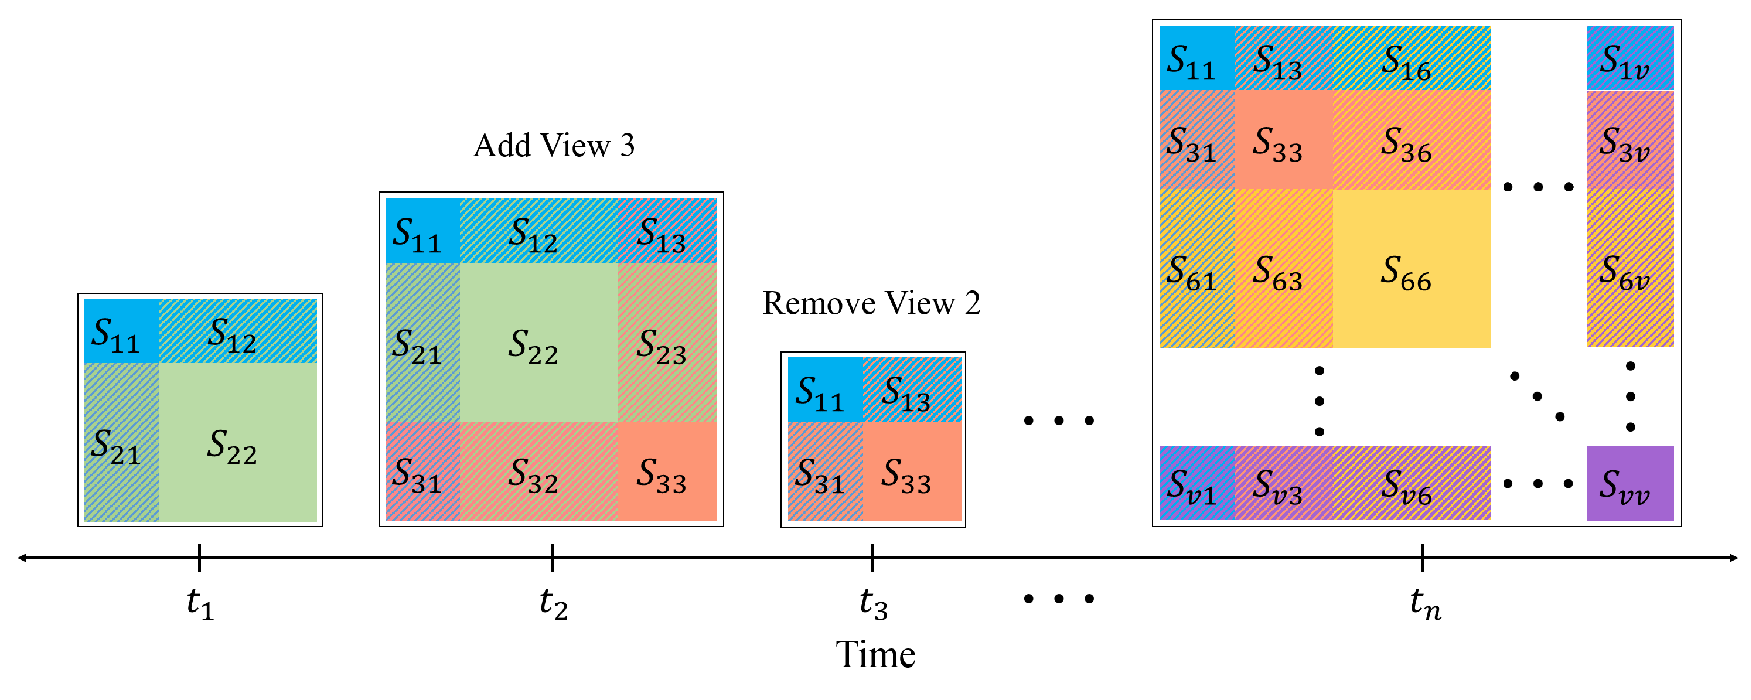
\includegraphics[width=0.9\textwidth]{Figures/VIDMvDA/Fig1.pdf}
	\caption{Updates in a scatter matrix after the addition and deletion of views over time. Each submatrix $\textbf{S}_{jr}$ is represented with the combination of colors of $j^{th}$ and $r^{th}$ view.}
	\label{fig:VIDMvDA_IncViews}
\end{figure*}

Fig. \ref{fig:VIDMvDA_IncViews} presents an example of updates in the scatter matrix with the increments or decrements in a pictorial form. In this figure, we see that at time $t_1$, there exists a within-class scatter matrix of two views. When a new view $3$ is added at the transition from $t_1$ to $t_2$,

\begin{itemize}
	\item The submatrices pertaining to the third view ($\textbf{S}_{13}, \textbf{S}_{23}, \textbf{S}_{31}$, $\textbf{S}_{32}$ and $\textbf{S}_{33}$) are appended to the scatter matrix from $t_1$ as shown in Fig. \ref{fig:VIDMvDA_IncViews}.
	\item The existing submatrices from $t_1$ ($\textbf{S}_{11}, \textbf{S}_{12}, \textbf{S}_{21}$ and $\textbf{S}_{22}$) are updated in $t_2$ to reflect the addition of the new view.
\end{itemize}
When view $2$ is deleted at the transition from $t_2$ to $t_3$,
\begin{itemize}
	\item The submatrices pertaining to the second view ($\textbf{S}_{12}, \textbf{S}_{21}$, $\textbf{S}_{22}, \textbf{S}_{23}$ and $\textbf{S}_{32}$) from $t_2$ are deleted at $t_3$.
	\item The remaining submatrices ($\textbf{S}_{11}, \textbf{S}_{13}, \textbf{S}_{31}$ and $\textbf{S}_{33}$) from $t_2$ are updated at $t_3$ to reflect the deletion of the view.
\end{itemize}
Following similar procedures for adding and deleting more views, we see the evolved scatter matrix at $t_n$.






\subsection{Addition of Views}
\label{sub:VIDMvDA_Add_View}
Let the set of new views be denoted as $\bar{\mathcal{V}} = \{ v+1, v+2, \cdots, v' \}$. When new views are added, four quantities are updated, namely- (i) data sample counts, (ii) the means, (iii) the within-class scatter and (iv) the between-class scatter. These updates are given as follows:

\subsubsection{Updating the number of data samples}
\label{ssubs:VIDMvDA_Inc_n}
As each of the new views contains features of all the existing data samples, the cardinality of each new view is the same as any previous view. Hence, the \textit{number of samples per class per view} ($n_{ij}'$) is also the same as that of any previous views. Other counts $n_i$ and $n$ are updated as follows,

\begin{equation}
\label{eqn:VIDMvDA_Add_n}
n'_i = n_i + \sum\limits_{j=v+1}^{v'} n_{ij}' \hspace{0.3cm} \text{and} \hspace{0.3cm} n' = n + \sum\limits_{i=1}^{c} \sum\limits_{j=v+1}^{v'} n'_{ij}
\end{equation}





\subsubsection{Updating the means}
\label{ssubs:VIDMvDA_Inc_mu}
The three means ($\textbf{m}_{ij}$, $\textbf{m}_{i}$, $\textbf{m}$) are updated as follows,

\begin{equation}
\label{eqn:VIDMvDA_Add_mu_ij}
{\textbf{m}'_{ij}}^{(\textbf{x})} = {\bar{\textbf{m}}_{ij}}^{(\textbf{x})} = \frac{1}{\bar{n}_{ij}} \sum\limits_{k=1}^{\bar{n}_{ij}} \bar{\textbf{x}}_{ijk}
\end{equation}

\begin{equation}
\label{eqn:VIDMvDA_Add_mu_i}
\textbf{m}'_{i} = \frac{n_i \; \textbf{m}_{i} + \bar{n}_i \; \bar{\textbf{m}}_i}{n_i'}
\end{equation}

\begin{equation}
\label{eqn:VIDMvDA_Add_mu}
\textbf{m}' = \frac{n \; \textbf{m} + \bar{n} \; \bar{\textbf{m}}}{n'}
\end{equation}





\subsubsection{Updating the within-class scatter}
\label{ssubs:VIDMvDA_Inc_Sw}
The new scatter matrix is the summation of the scatter of the old and the new view with respect to the updated class mean. The equation to update within-class scatter is as follows,

\begin{equation}
\label{eqn:Add_Sw}
\mathbf{S}_W' = \sum_{i=1}^{c} \sum_{j=1}^{v} \sum_{k=1}^{n_{ij}} \left ( \mathbf{y}_{ijk} - \textbf{m}'_i \right ) \left ( \mathbf{y}_{ijk} - \textbf{m}'_i \right )^T + \sum_{i=1}^{c} \sum_{j=v+1}^{v'} \sum_{k=1}^{\bar{n}_{ij}} \left ( \bar{\mathbf{y}}_{ijk} - \textbf{m}'_i \right ) \left ( \bar{\mathbf{y}}_{ijk} - \textbf{m}'_i \right )^T\\
\end{equation}

This equation is in the projected space. We then express it only in terms of the old scatter matrix and new data in the original space. Here, we compute the submatrices ($\textbf{S}_{jr}$) of the within-class scatter of the new view with existing views in a pair-wise manner. Also, the existing submatrices are updated to reflect the change in the \textit{number of samples per class}. So, we have three cases based on the values of $j$ and $r$. At the transition from $t_1$ to $t_2$ in Fig. \ref{fig:VIDMvDA_IncViews}, we see these three cases.
\begin{itemize}
	\item \textit{Case-1} is when ($j \in \bar{\mathcal{V}} \;\;\&\&\;\; r \in \bar{\mathcal{V}}$), but ($j \neq r$). This case is for computing the scatter of new views with the existing views. In Fig. \ref{fig:VIDMvDA_IncViews}, submatrices $\textbf{S}_{13}, \textbf{S}_{23}, \textbf{S}_{31}$ and $\textbf{S}_{32}$ at $t_2$ represent this case.
	\item \textit{Case-2} is when ($j \in \bar{\mathcal{V}} \;\;\&\&\;\; r \in \bar{\mathcal{V}}$) and ($j = r$), that is when we compute the scatter of the new view with respect to itself. Submatrix $\textbf{S}_{33}$ at $t_2$ represents this case in Fig. \ref{fig:VIDMvDA_IncViews}.
	\item \textit{Case-3} is for updating the existing submatrices, which occurs when $(j \notin \bar{\mathcal{V}} \;\;\&\&\;\; r \notin \bar{\mathcal{V}})$. Submatrices $\textbf{S}_{11}, \textbf{S}_{12}$, $\textbf{S}_{21}$ and $\textbf{S}_{22}$ at $t_2$ in Fig. \ref{fig:VIDMvDA_IncViews} represent \textit{Case-3}.
\end{itemize}


The equation for updating the within-class scatter matrix in all three cases is given below.

\begin{equation}
\label{eqn:VIDMvDA_Add_Sjr}
\begin{split}
\textbf{S}_{jr}' = \left\{\begin{matrix*}[l]
- \sum\limits_{i=1}^{c} \frac{\bar{n}_{ij} \bar{n}_{ir}}{n_i'} \; {\textbf{m}_{ij}}^{(\textbf{x})} \; {\textbf{m}_{ir}}^{(\textbf{x})^T} & \text{case 1}
\\[0.4cm]
\sum\limits_{i=1}^{c} \bigg[ \sum\limits_{k=1}^{\bar{n}_{ij}} \bar{\textbf{x}}_{ijk} {\bar{\textbf{x}}_{ijk}}^T - \frac{\bar{n}_{ij} \bar{n}_{ij}}{n_i'} \; {\textbf{m}_{ij}}^{(\textbf{x})} \;{\textbf{m}_{ij}}^{(\textbf{x})^T} \bigg] & \text{case 2}
\\[0.4cm]
\textbf{S}_{jr} + \sum\limits_{i=1}^{c}  \frac{n_i' - n_i}{n_i n_i'} \; n_{ij} n_{ir} \; {\textbf{m}_{ij}}^{(\textbf{x})} {\textbf{m}_{ir}}^{(\textbf{x})^T} & \text{case 3}
\end{matrix*}\right.
\end{split}
\end{equation}

The derivation of $\textbf{S}_{W}'$ and $\textbf{S}_{jr}'$ is given in Appendix-G.%\ref{proof:VIDMvDA_Sjr}.





\begin{algorithm}[t]
\centering
\caption{VIDMvDA: Incremental algorithm}
\label{VIDMvDA_Algo_Add}
    \begin{algorithmic}
	\STATE \textbf{Input :}
	\STATE - An existing model $\phi$ that consists of $n$, $n_i$, $n_{ij}$, $\textbf{m}_{ij}^{(\textbf{x})}$, $\textbf{S}$, $\textbf{D}$, $\mathcal{C}$, $\mathcal{V}$
	\STATE 		- New views of data samples: $\bar{\mathcal{X}}$
	\STATE 		- Set of new views: $\bar{\mathcal{V}}$ \vspace{0.1cm}

	\WHILE{new data is encountered}
		
		\STATE \small Update $n$, $n_i$, $n_{ij}$ as given in Eq.\ref{eqn:VIDMvDA_Add_n}\;
		\STATE \small Update mean per class per view $(\textbf{m}_{ij}^{(\textbf{x})})$ using Eq.\ref{eqn:VIDMvDA_Add_mu_ij}\;
		\STATE \small Update the within-class scatter matrix $(\textbf{S})$ using Eq.\ref{eqn:VIDMvDA_Add_Sjr}\;
		\STATE \small Update the between-class scatter matrix $(\textbf{D})$ using Eq.\ref{eqn:VIDMvDA_Add_Djr}\;
		\STATE $\mathcal{V} = \mathcal{V} \cup \bar{\mathcal{V}}$ \;
			
		\STATE \small Calculate the projection matrix $(\textbf{W}^{opt})$ using Eq.\ref{eqn:Lit_MvDA_GEP}\;
	\ENDWHILE
	\STATE \textbf{Output :}
	\STATE - Updated model $\phi'$ and the projection matrix $\textbf{W}^{opt}$

\end{algorithmic}
\end{algorithm}





\subsubsection{Updating the between-class scatter}
\label{ssubs:VIDMvDA_Inc_Sb}
The between-class scatter depends only on the means, so updating the between-class scatter after each increment is easier. The equation in projected space does not explicitly depend on the views.

\begin{equation}
\label{eqn:VIDMvDA_Add_Sb}
\textbf{S}_B' = \; \sum_{i=1}^{c} n_{i}' (\textbf{m}_{i}' - \textbf{m}') (\textbf{m}_{i}' - \textbf{m}')^T
\end{equation}

Here, the view information is embedded in the total and class-wise means. It creates two cases of updates when rewritten using the data samples in the original space.

In \textit{Case-1}, the between-class scatter of the new views with the existing views is computed in a pairwise manner and appended to the existing scatter matrix ($\textbf{D}$). Here, ($ j \in \bar{\mathcal{V}} \;\; || \;\; r \in \bar{\mathcal{V}}$). In \textit{Case-2}, all the existing submatrices are adjusted to reflect the change in the means and the number of data samples. Here, ($ j \notin \bar{\mathcal{V}} \;\; \&\& \;\; r \notin \bar{\mathcal{V}}$). The update equations for both the cases of the between-class scatter are as follows,


\begin{equation}
\label{eqn:VIDMvDA_Add_Djr}
\textbf{D}_{jr}' = \left\{\begin{matrix*}[l]
\sum\limits_{i=1}^{c} \frac{n'_{ij} \; n'_{ir}}{n'_i} \; {\textbf{m}'_{ij}}^{(\textbf{x})} \; {\textbf{m}'_{ir}}^{(\textbf{x})^T} - \frac{1}{n'} \left ( \sum\limits_{i=1}^{c} n'_{ij} \; {\textbf{m}'_{ij}}^{(\textbf{x})} \right )\left ( \sum\limits_{i=1}^{c} n'_{ir} \; {\textbf{m}'_{ir}}^{(\textbf{x})} \right )^T & \text{case 1}
\\
\textbf{D}_{jr} - \sum\limits_{i=1}^{c} \frac{n_i' - n_i}{n_i \; n_i'} \; n_{ij} \; n_{ir} {\textbf{m}_{ij}}^{(\textbf{x})} \; {\textbf{m}_{ir}}^{(\textbf{x})^T} + \frac{n' - n}{n \; n'} \left ( \sum\limits_{i=1}^{c} n_{ij} \; {\textbf{m}_{ij}}^{(\textbf{x})} \right )\left ( \sum\limits_{i=1}^{c} n_{ir} \; {\textbf{m}_{ir}}^{(\textbf{x})} \right )^T & \text{case 2}
\end{matrix*}\right.
\end{equation}

The derivation of $\textbf{S}_{B}'$ and $\textbf{D}_{jr}'$ is given in Appendix-A%\ref{proof:Djr}
. After performing steps (i)-(iv), we compute the optimal projection matrix by solving the generalized eigenvalue problem given in Eq. \ref{eqn:Lit_MvDA_GEP}. The obtained projection matrix ($\textbf{W}^{opt}$) is then used for classification by projecting each test sample onto a shared subspace where they can be assigned labels based on their proximity to the available classes. This projection matrix is used until further addition or deletion of the views. Whenever we encounter yet another new view/s of the data, we repeat the update process and compute the new projection matrix. The whole process is summarized in Algorithm \ref{VIDMvDA_Algo_Add}. This formulation can be used for 2D data as well.







\subsection{Deletion of Views}
\label{sub:VIDMvDA_Del_View}
Let $\bar{\mathcal{V}} \subset \mathcal{V}$ be a set of $\bar{v}$ views to be removed from the dataset. When any of the existing views are deleted, four quantities, namely (i) the data sample counts, (ii) the means, (iii) the within-class scatter, and (iv) the between-class scatter. These updates are given as follows:


\subsubsection{Updating the number of data samples}
\label{ssubs:VIDMvDA_Dec_n}
As these views of all existing data samples are deleted, the \textit{number of data samples per class per view} ($n_{ij}'$) of each of these views will also be deleted or made equal to $0$. The \textit{number of data samples per class} ($n_i$), and the \textit{total number of data samples} ($n$) are updated as,

\begin{equation}
\label{eqn:VIDMvDA_Del_n}
n'_i = n_i - \sum\limits_{j=1}^{\bar{v}} n_{ij} \hspace{0.3cm} \text{and} n' = n - \sum\limits_{i=1}^{c} \sum\limits_{j=1}^{\bar{v}} n_{ij}
\end{equation}




\subsubsection{Updating the means}
\label{ssubs:VIDMvDA_Dec_mu}
The three means ($\textbf{m}_{ij}$, $\textbf{m}_{i}$, $\textbf{m}$) are updated as follows,

\begin{equation}
\label{eqn:VIDMvDA_Del_mu_ij}
{\textbf{m}'_{ij}}^{(\textbf{x})} = 0
\end{equation}

\begin{equation}
\label{eqn:VIDMvDA_Del_mu_i}
\textbf{m}'_{i} = \frac{n_i \; \textbf{m}_{i} - \bar{n}_i \; \bar{\textbf{m}}_i}{n_i'}
\end{equation}

\begin{equation}
\label{eqn:VIDMvDA_Del_mu}
\textbf{m}' = \frac{n \; \textbf{m} - \bar{n} \; \bar{\textbf{m}}}{n'}
\end{equation}




\begin{algorithm}[t]
\centering
\caption{VIDMvDA: Decremental algorithm}
\label{VIDMvDA_Algo_Del}
    \begin{algorithmic}
	\STATE \textbf{Input :}
	\STATE - An existing model $\phi$ that consists of $n$, $n_i$, $n_{ij}$, $\textbf{m}_{ij}^{(\textbf{x})}$, $\textbf{S}$, $\textbf{D}$, $\mathcal{C}$, $\mathcal{V}$
	\STATE 		- Views of data samples to be removed: $\bar{\mathcal{X}}$
	\STATE 		- Set of views to be removed: $\bar{\mathcal{V}}$ \vspace{0.1cm}

	\WHILE{there is a view is to be removed}
		
		\STATE \small Update $n$, $n_i$, $n_{ij}$ as given in \ref{eqn:VIDMvDA_Del_n}\;
		\STATE \small Update mean per class per view $(\textbf{m}_{ij}^{(\textbf{x})})$ using Eq.\ref{eqn:VIDMvDA_Del_mu_ij}\;
		\STATE \small Update the within-class scatter matrix $(\textbf{S})$ using Eq.\ref{eqn:VIDMvDA_Del_Sjr}\;
		\STATE \small Update the between-class scatter matrix $(\textbf{D})$ using Eq.\ref{eqn:VIDMvDA_Del_Djr}\;
		\STATE $\mathcal{V} = \mathcal{V} - \bar{\mathcal{V}}$ \;
			
		\STATE \small Calculate the projection matrix $(\textbf{W}^{opt})$ using Eq.\ref{eqn:Lit_MvDA_GEP}\;
	\ENDWHILE
	\STATE \textbf{Output :}
	\STATE - Updated model $\phi'$ and the projection matrix $\textbf{W}^{opt}$

\end{algorithmic}
\end{algorithm}





\subsubsection{Updating the within-class scatter}
\label{ssubs:VIDMvDA_Dec_Sw}
The new scatter matrix is the summation of the scatter of the remaining data samples from the updated class mean. The equation in the projected space is as follows,

\begin{equation}
\label{eqn:VIDMvDA_Del_Sw}
\mathbf{S}_W' = \sum_{i=1}^{c} \sum_{j=1}^{v} \sum_{k=1}^{n_{ij}} \left ( \mathbf{y}_{ijk} - \textbf{m}'_i \right ) \left ( \mathbf{y}_{ijk} - \textbf{m}'_i \right )^T - \sum_{i=1}^{c} \sum_{j=1}^{\bar{v}} \sum_{k=1}^{\bar{n}_{ij}} \left ( \bar{\mathbf{y}}_{ijk} - \textbf{m}'_i \right ) \left ( \bar{\mathbf{y}}_{ijk} - \textbf{m}'_i \right )^T
\end{equation}

This equation is in the projected space. In the original space, we delete all the submatrices ($\textbf{S}_{jr}$) of the within-class scatter that pertain to the views to be deleted. The remaining submatrices are updated to reflect the change in the \textit{number of samples per class}. Here, we have two cases based on the values of $j$ and $r$. For example, at the transition from $t_2$ to $t_3$ in Fig. \ref{fig:VIDMvDA_IncViews}, we see these two cases.
\begin{itemize}
	\item \textit{Case-1} is when either ($j \in \bar{\mathcal{V}} \;\;||\;\; r \in \bar{\mathcal{V}}$). This case is for deleting the pairwise scatter of views in $\bar{\mathcal{V}}$ with any other view. Submatrices $\textbf{S}_{12}, \textbf{S}_{21}, \textbf{S}_{22}, \textbf{S}_{23}$ and $\textbf{S}_{32}$ from time-stamp $t_2$ are deleted from the scatter matrix at $t_3$ in Fig. \ref{fig:VIDMvDA_IncViews}.
	\item \textit{Case-2} is for updating the existing submatrices. This occurs when $(j \notin \bar{\mathcal{V}} \;\;\&\&\;\; r \notin \bar{\mathcal{V}})$. Submatrices $\textbf{S}_{11}, \textbf{S}_{13}, \textbf{S}_{31}$ and $\textbf{S}_{33}$ at $t_3$ represent \textit{Case-2} in Fig. \ref{fig:VIDMvDA_IncViews}.
\end{itemize}

The within-class scatter matrix is updated as follows-

\begin{equation}
\label{eqn:VIDMvDA_Del_Sjr}
\begin{split}
\textbf{S}_{jr}' = \left\{\begin{matrix*}[l]
Delete & \text{case 1}
\\[0.4cm]
\textbf{S}_{jr} + \sum\limits_{i=1}^{c}  \frac{n_i' - n_i}{n_i n_i'} \; n_{ij} n_{ir} \; {\textbf{m}_{ij}}^{(\textbf{x})} {\textbf{m}_{ir}}^{(\textbf{x})^T} & \text{case 2}
\end{matrix*}\right.
\end{split}
\end{equation}

The derivation of $\textbf{S}_{W}'$ and $\textbf{S}_{jr}'$ is the same as in the case of incremental formulation given in Appendix-G.%\ref{proof:VIDMvDA_Sjr}.




\subsubsection{Updating the between-class scatter}
\label{ssubs:VIDMvDA_Dec_Sb}
As we have seen in the case of increment, the equation of between-class scatter in projected space does not explicitly depend on the views.

\begin{equation}
\label{eqn:VIDMvDA_Del_Sb}
\textbf{S}_B' = \; \sum_{i=1}^{c} n_{i}' (\textbf{m}_{i}' - \textbf{m}') (\textbf{m}_{i}' - \textbf{m}')^T
\end{equation}

The between-class scatter also has the same two cases as the within-class scatter in the original space. For \textit{case-1}, the submatrices pertaining to the views in set $\bar{\mathcal{V}}$ are deleted. For \textit{case-2}, the submatrices are updated as follows,

\small
\begin{equation}
\label{eqn:VIDMvDA_Del_Djr}
\begin{split}
\textbf{D}_{jr}' = \left\{\begin{matrix*}[l]
Delete & \text{case 1}
\\[0.4cm]
\sum\limits_{i=1}^{c} \frac{n'_{ij} \; n'_{ir}}{n'_i} \; {\textbf{m}_{ij}}^{(\textbf{x})} \; {\textbf{m}_{ir}}^{(\textbf{x})^T} - \frac{1}{n'} \left ( \sum\limits_{i=1}^{c} n'_{ij} \; {\textbf{m}_{ij}}^{(\textbf{x})} \right )\left ( \sum\limits_{i=1}^{c} n'_{ir} \; {\textbf{m}_{ir}}^{(\textbf{x})} \right )^T & \text{case 2}
\end{matrix*}\right.
\end{split}
\end{equation}
\normalsize

The derivation of $\textbf{S}_{B}'$ and $\textbf{D}_{jr}'$ is given in Appendix-A.%\ref{proof:Djr}.

After following steps (i)-(iv), we compute the optimal projection matrix using Eq. \ref{eqn:Lit_MvDA_GEP}. The projection matrix ($\textbf{W}^{opt}$), thus obtained, is then used until a new view of the data arrives or any of the existing view/s are deleted. While deleting another view/s of the data, we repeat the update process presented above and compute the new projection matrix. The whole process is summarized in Algorithm \ref{VIDMvDA_Algo_Del}. This formulation can be used for 2D data as well.










\section{Experiments and Results}
\label{sec:VIDMvDA_Expt}

\subsection{Experimental Setup}
\label{subs:VIDMvDA_Expt_Setup}
We have divided the data samples from each dataset into two subsets- one for training (80\%) and the other as a test set (20\%). The training set is used to simulate the increments and decrements of views. Though VIDMvDA can handle one or more views of data in each increment or decrement, to demonstrate the effect of adding the views, we have used the views one at a time for the experiments.

For experiments with 1D datasets, two models, $\phi_A$ and $\phi_B$, are trained on each dataset. $\phi_A$ is trained using VIDMvDA, and $\phi_B$ is trained using the 1D batch method, MvDA. While simulating the increments, we add one view at a time from 1 to 6. VIDMvDA updates $\phi_A$ by considering only the old model and the new view after each increment, whereas MvDA discards $\phi_B$ and trains a new model after each increment using all the existing views and the new view. After both models have been trained on all views of the dataset, we simulate decrement by removing one view at a time from 1 to 5. While simulating the decrement, $\phi_A$ is updated to reflect the deletion of each view using only the existing model, whereas $\phi_B$ is discarded and trained anew using all the remaining views after the deletion.

% Reviewer
For experiments with 2D datasets, two models, $\phi_A$ and $\phi_B$, are trained on each dataset. $\phi_A$ is trained using VIDMvDA, and $\phi_B$ is trained using the 2D batch method, 2DMvDA. The increments and decrements are simulated in a similar way as with the 1D datasets.

The updated models after each increment/decrement are used to classify the data samples from the test set. Here, only the views used in the training phase of that time step are taken into account. Let $\textbf{W}^{opt}_A$ and $\textbf{W}^{opt}_B$ be the optimal projection matrices obtained from models $\phi_A$ and $\phi_B$, respectively. The projection matrix from each method is then used to project every test sample ($\textbf{y}^{Test}$) onto the shared space. We use the same methodology as that used by MvIDA for classification.






\subsection{Results}
\label{subs:VIDMvDA_Res}
This section presents the results of experiments designed in order to answer the research questions posed in chapter \ref{ch:Intro}.


\subsubsection{Similarity of the Discriminative Subspace}
\label{ssubs:VIDMvDA_Subspace}
\begin{itemize}
\item \textbf{RQ1 :}
Can the incremental-decremental method, without using old views, produce an identical model to that of its batch counterpart?

\item \textbf{Experiment :}
We train two models using VIDMvDA and its batch counterpart to compare the discriminant subspace. We first incrementally learn all views one by one and then unlearn those in a similar fashion. The inner product of projection vectors of these methods is taken after each update.

\item \textbf{Discussion :}
Fig. \ref{fig:VIDMvDA_Res_Subspace} presents the inner product of projection vectors obtained from the models trained on handwritten digits dataset. The results on all the other datasets are similar to those presented in this figure. Hence, no separate results are presented. We see the inner product of projection vectors after adding each view incrementally from $1$ to $6$. The figure also shows the inner product after removing them in the same order from $1$ to $5$. After the deletion of the $6^{th}$ view, the scatter matrices become zero. Here, the labels EV1 to EV5 represent the first five projection vectors and the number of the added/deleted view is written on the x-axis. We see that the inner product of projection vectors is either $1$ or very close to $1$ even after the addition of new views. The same observation is made for the deletion operation. This observation shows that the discriminant subspace constructed by VIDMvDA is nearly identical to that of the its batch counterparts, MvDA or 2DMvDA.
\end{itemize}




\begin{figure}[t]
	\centering
	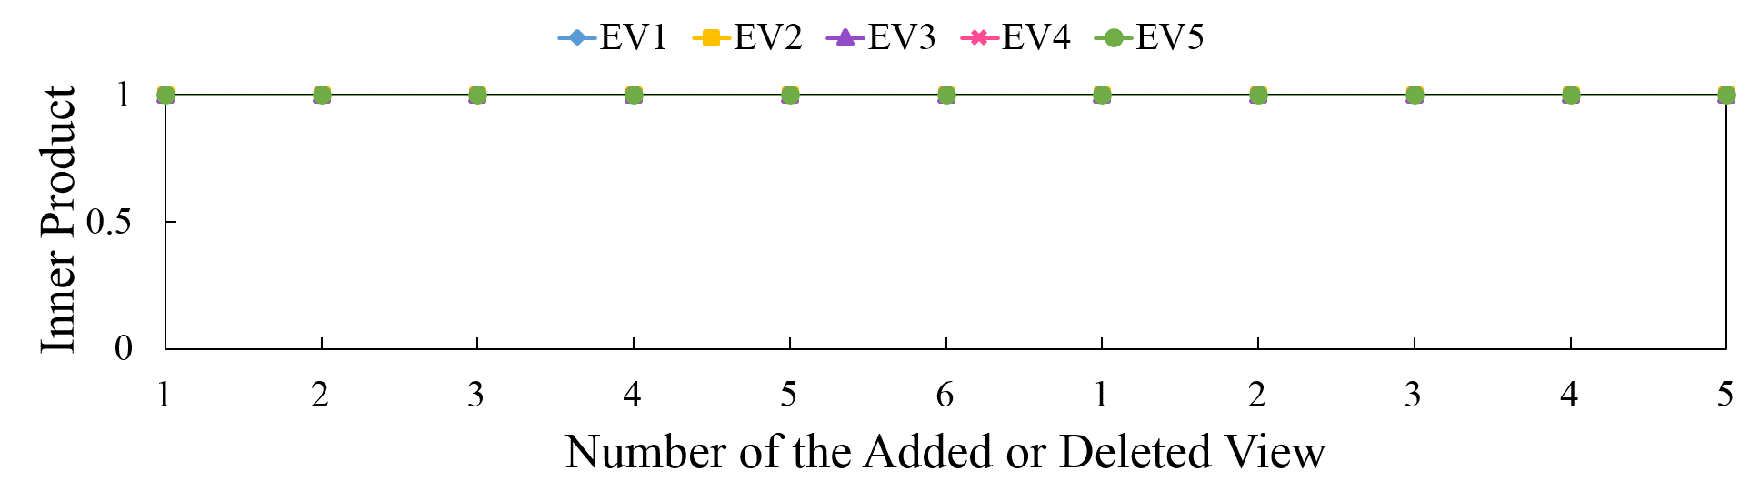
\includegraphics[width=\textwidth]{Figures/VIDMvDA/Fig2.pdf}
	\caption{Inner products of the first five projection vectors of VIDMvDA and MvDA on handwritten digits dataset. Views are added to the initially empty dataset one by one from 1 to 6. After that, they are removed from the dataset in the order from 1 to 5.}
	\label{fig:VIDMvDA_Res_Subspace}
\end{figure}




\begin{figure}[t]
	\centering
	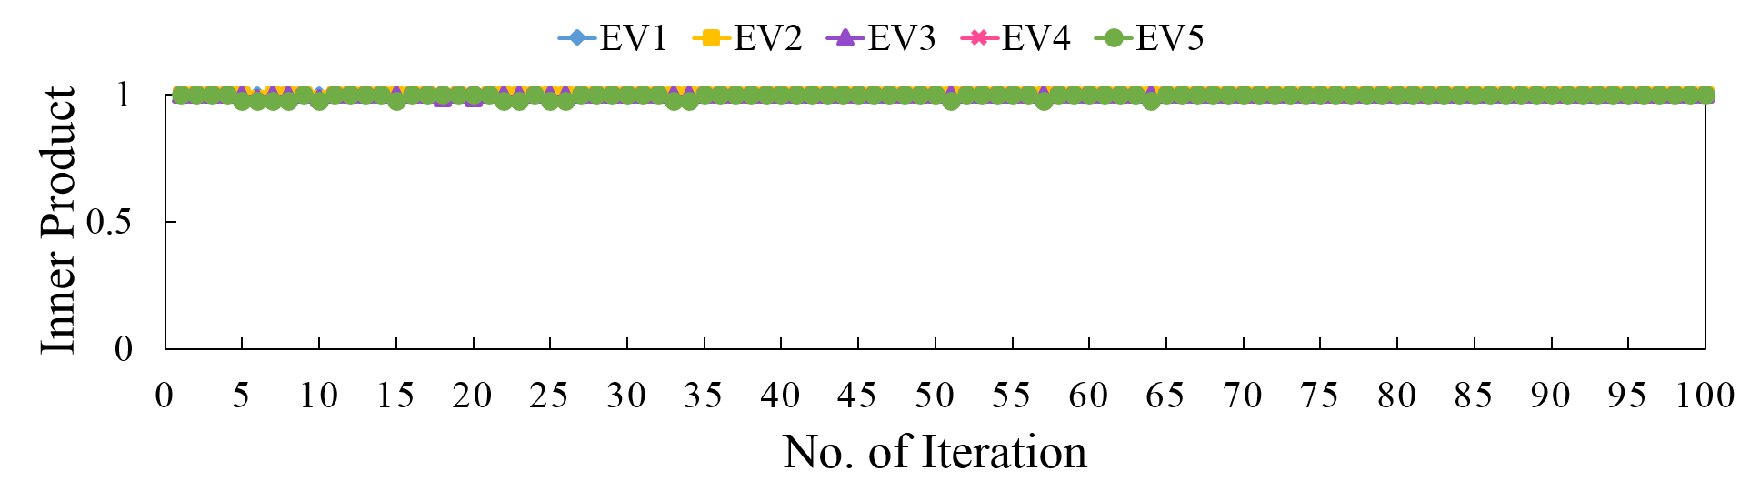
\includegraphics[width=\textwidth]{Figures/VIDMvDA/Fig3.pdf}
	\caption{Inner products of the first five projection vectors of 100 iterations of VIDMvDA with those of MvDA on handwritten digits dataset.}
	\label{fig:VIDMvDA_Res_OI}
\end{figure}




\subsubsection{Order Independence}
\label{ssubs:VIDMvDA_OI}
\begin{itemize}
\item \textbf{RQ2 :}
Is this method invariant to the order of addition or deletion of data samples?

\item \textbf{Experiment :}
We trained a hundred models using VIDMvDA on the training set by adding or deleting the data samples in a randomized order every time. When the updates are done after each iteration, we compute the inner product of the eigenvectors of the trained model with the eigenvectors of the batch method, MvDA for 1D datasets or 2DMvDA for 2D datasets.

\item \textbf{Discussion :}
We use the inner product of projection vectors to check whether the subspace constructed by VIDMvDA is similar to that constructed by a batch method. Here, we have only shown the results obtained on the Handwritten Digits dataset to avoid redundancy. We see in Fig. \ref{fig:VIDMvDA_Res_OI} that the values of the inner product of the projection vectors have converged to $1$ regardless of the order of addition or deletion of views, demonstrating the order independence of VIDMvDA.
\end{itemize}









\subsubsection{Comparison of Classification Accuracy}
\label{ssubs:VIDMvDA_Acc}
\begin{table*}[t]
	\centering
	\caption{Comparison of the classification accuracy of VIDMvDA and MvDA. First column shows the number of the view that was added or deleted.}
	\label{tab:VIDMvDA_Res_Acc}
	\begin{tabular}{l r l r l r l} \hline
		View & \multicolumn{2}{c}{\textbf{Handwritten Digits}} & \multicolumn{2}{c}{\textbf{Caltech-7}} & \multicolumn{2}{c}{\textbf{AwA}} \\
		No. & \textbf{VIDMvDA} & \textbf{MvDA} & \textbf{VIDMvDA} & \textbf{MvDA} & \textbf{VIDMvDA} & \textbf{MvDA} \\ \hline
		\multicolumn{7}{c}{\textbf{Addition of Views}} \\ \hline
		1 &  98.25 \hspace{0.5cm} & 96.75 & 89.00 \hspace{0.5cm} & 89.00 & 90.69 \hspace{0.5cm} & 90.69 \\ 
		2 &  98.75 \hspace{0.5cm} & 92.00 & 90.00 \hspace{0.5cm} & 90.00 & 94.43 \hspace{0.5cm} & 94.43 \\ 
		3 &  98.00 \hspace{0.5cm} & 97.25 & 92.50 \hspace{0.5cm} & 92.50 & 94.27 \hspace{0.5cm} & 94.27 \\ 
		4 & 100.00 \hspace{0.5cm} & 99.00 & 96.00 \hspace{0.5cm} & 96.00 & 94.43 \hspace{0.5cm} & 92.79 \\ 
		5 & 100.00 \hspace{0.5cm} & 98.75 & 97.00 \hspace{0.5cm} & 97.00 & 95.43 \hspace{0.5cm} & 95.43 \\ 
		6 &  99.75 \hspace{0.5cm} & 99.00 & 97.00 \hspace{0.5cm} & 97.00 & 96.55 \hspace{0.5cm} & 96.55 \\ \hline

		\multicolumn{7}{c}{\textbf{Deletion of Views}} \\ \hline
		1 & 100.00 \hspace{0.5cm} & 99.00 & 97.00 \hspace{0.5cm} & 97.00 & 96.55 \hspace{0.5cm} & 96.55 \\ 
		2 & 100.00 \hspace{0.5cm} & 98.75 & 95.50 \hspace{0.5cm} & 95.50 & 96.02 \hspace{0.5cm} & 95.73 \\ 
		3 &  98.75 \hspace{0.5cm} & 98.75 & 96.50 \hspace{0.5cm} & 96.50 & 96.02 \hspace{0.5cm} & 96.02 \\ 
		4 & 100.00 \hspace{0.5cm} & 97.00 & 96.00 \hspace{0.5cm} & 96.00 & 94.88 \hspace{0.5cm} & 94.88 \\ 
		5 & 100.00 \hspace{0.5cm} & 98.75 & 96.00 \hspace{0.5cm} & 96.00 & 93.36 \hspace{0.5cm} & 93.36 \\ \hline
	
	\end{tabular}
\end{table*}

\begin{table*}[t]
	\centering
	\caption{Comparison of the classification accuracy of VIDMvDA and MvDA. First column shows the number of the view that was added or deleted.}
	\label{tab:VIDMvDA_Res_Acc_2D}
	\begin{tabular}{l r l r l r l r l} \hline
		View & \multicolumn{2}{c}{\textbf{IMPART}} & \multicolumn{2}{c}{\textbf{MSSpoof}} & \multicolumn{2}{c}{\textbf{Stereo Face}} & \multicolumn{2}{c}{\textbf{ORL}} \\
		No. & \textbf{\footnotesize{VIDMvDA}} & \textbf{\footnotesize{2DMvDA}} & \textbf{\footnotesize{VIDMvDA}} & \textbf{\footnotesize{2DMvDA}} & \textbf{\footnotesize{VIDMvDA}} & \textbf{\footnotesize{2DMvDA}} & \textbf{\footnotesize{VIDMvDA}} & \textbf{\footnotesize{2DMvDA}} \\ \hline
		\multicolumn{9}{c}{\textbf{Addition of Views}} \\ \hline
		1 & 100.00 \hspace{0.5cm} & 100.00 & 97.33 \hspace{0.5cm} & 97.33 & 95.00 \hspace{0.5cm} & 95.00 & 90.00 \hspace{0.5cm} & 90.00 \\ 
		2 & 90.00 \hspace{0.5cm} & 90.00 & 100.00 \hspace{0.5cm} & 98.67 & 98.12 \hspace{0.5cm} & 98.12 & 87.50 \hspace{0.5cm} & 87.50 \\ 
		3 & 100.00 \hspace{0.5cm} & 100.00 & - \hspace{0.5cm} & - & - \hspace{0.5cm} & - & 91.25 \hspace{0.5cm} & 91.25 \\ 
		4 & 100.00 \hspace{0.5cm} & 100.00 & - \hspace{0.5cm} & - & - \hspace{0.5cm} & - & - \hspace{0.5cm} & - \\ 
		5 & 100.00 \hspace{0.5cm} & 100.00 & - \hspace{0.5cm} & - & - \hspace{0.5cm} & - & - \hspace{0.5cm} & - \\ \hline

		\multicolumn{9}{c}{\textbf{Deletion of Views}} \\ \hline
		1 & 100.00 \hspace{0.5cm} & 100.00 & 100.00 \hspace{0.5cm} & 100.00 & 97.50 \hspace{0.5cm} & 97.50 & 93.75 \hspace{0.5cm} & 93.75 \\ 
		2 & 100.00 \hspace{0.5cm} & 100.00 & - \hspace{0.5cm} & - & - \hspace{0.5cm} & - & 78.75 \hspace{0.5cm} & 78.75 \\ 
		3 & 100.00 \hspace{0.5cm} & 100.00 & - \hspace{0.5cm} & - & - \hspace{0.5cm} & - & - \hspace{0.5cm} & - \\ 
		4 & 100.00 \hspace{0.5cm} & 100.00 & - \hspace{0.5cm} & - & - \hspace{0.5cm} & - & - \hspace{0.5cm} & - \\ \hline
	
	\end{tabular}
\end{table*}

\begin{itemize}
\item \textbf{RQ3 :}
Can this method perform as well as the batch method in terms of classification accuracy?

\item \textbf{Experiment :}
We have noted the classification performance of the incremental and the batch methods after adding each view to the dataset and later removing them one by one.

\item \textbf{Discussion :}
Here, we have used 5 projection vectors, i.e. $d = 5$, for both the models $\phi_A$ and $\phi_B$. The results show that VIDMvDA has the same or better classification accuracy than its batch counterparts. Table \ref{tab:VIDMvDA_Res_Acc} presents the records of classification accuracies on 1D datasets

\begin{figure}[t]
\centering
  \begin{subfigure}[h]{0.48\textwidth}
    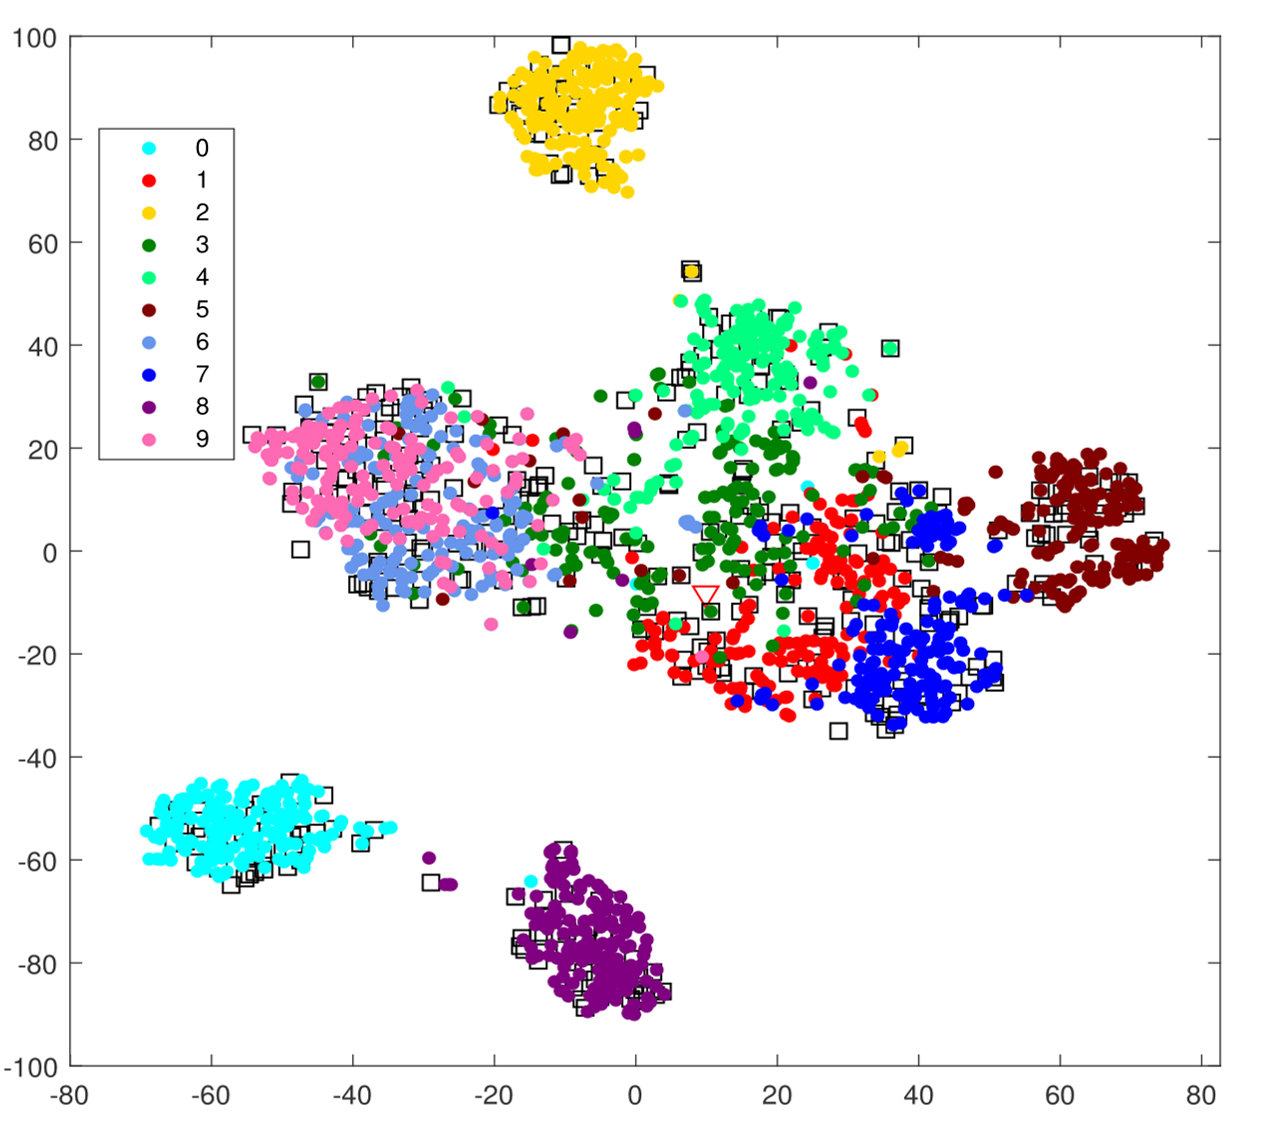
\includegraphics[width=\textwidth]{Figures/VIDMvDA/Fig4.png}
    \caption{{VIDMvDA}}
    \label{fig:VIDMvDA_Res_Vis_VIDMvDA}
  \end{subfigure}
  \begin{subfigure}[h]{0.48\textwidth}
    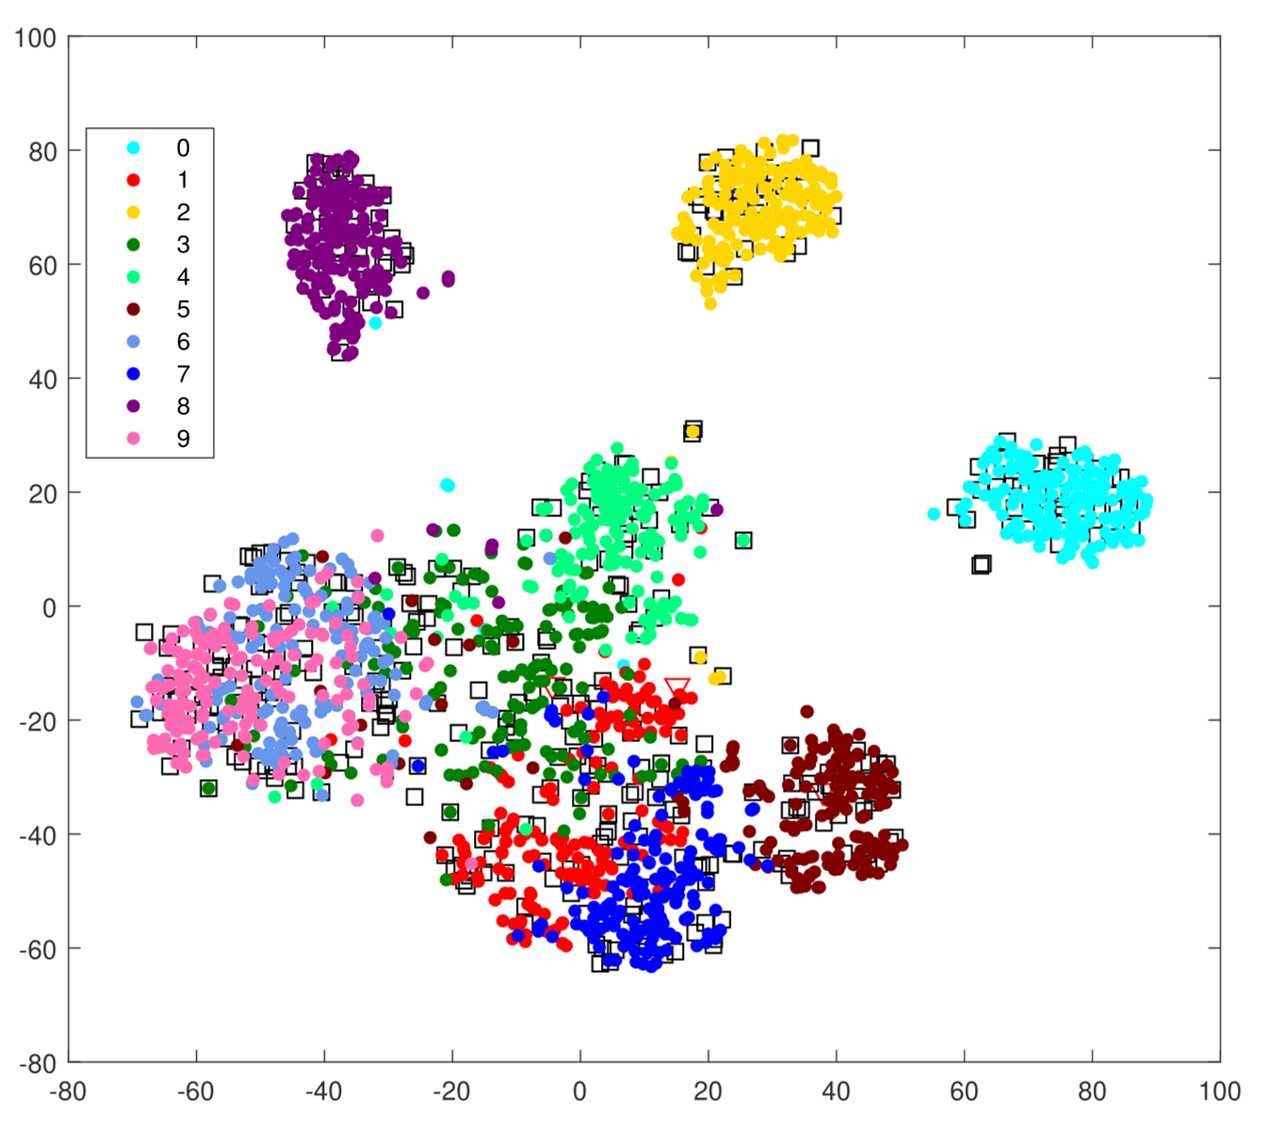
\includegraphics[width=\textwidth]{Figures/VIDMvDA/Fig5.png}
    \caption{{MvDA}}
    \label{fig:VIDMvDA_Res_Vis_MvDA}
  \end{subfigure}
\caption{A plot of data samples of the handwritten digits dataset in the projected space constructed by (a) VIDMvDA and (b) MvDA. Training data samples from different classes are shown in different colors. Black squares show correctly classified test samples, and red triangles show incorrectly classified test samples.}
\label{fig:VIDMvDA_Res_Vis}
\end{figure}
\clearpage


\noindent and Table \ref{tab:VIDMvDA_Res_Acc_2D} shows the records for 2D datasets. We saw in \ref{ssubs:VIDMvDA_Subspace}, that the discriminant subspaces of both models are very similar. The same is observed with the classification accuracy as well. The accuracy of these two models is the same for all the datasets, except for the handwritten digits dataset and MSSpoof dataset. VIDMvDA performs a little better than the batch methods on these datasets.
 
A t-SNE plot of handwritten digits dataset in the projected space constructed by VIDMvDA and MvDA is presented in Fig. \ref{fig:VIDMvDA_Res_Vis}. Here, 0 to 9 are the class labels. We see that both models project the data in a similar manner. Both methods have set classes 0, 2 and 8 (denoted with cyan, yellow and violet) farther from the other classes. Classes 6 and 9 (pink and sky-blue) are closer to each other, as are classes 1 and 7 (red and blue).
\end{itemize}








\subsubsection{Comparison of Training Time}
\label{ssubs:VIDMvDA_Time}
\begin{itemize}
\item \textbf{RQ4 :}
Can this method reduce training time?

\item \textbf{Experiment :}
To compare the training time of VIDMvDA and MvDA/2DMvDA, we trained models using these methods by adding the views in a one-by-one manner from view 1 to 6. Similarly, for deletion, the time was noted after each view was deleted from view 1 to 5. We record the time taken by each method after every addition/deletion of views.

\item \textbf{Discussion :}
As VIDMvDA only updates the existing model instead of retraining from scratch, it is expected to require less time for training than the batch method as the latter discards the existing model and retrains on the whole dataset. This observation is reflected in the recorded training time of these methods. Fig. \ref{fig:VIDMvDA_Res_Time_Add} and \ref{fig:VIDMvDA_Res_Time_Del} present the records of training time of the 1D datasets for increments and decrements, respectively. Similarly, Fig. \ref{fig:VIDMvDA_Res_Time_Add_2D} and \ref{fig:VIDMvDA_Res_Time_Del_2D} present the records for 2D datasets.

We see in Fig. \ref{fig:VIDMvDA_Res_Time_Add} and Fig. Fig. \ref{fig:VIDMvDA_Res_Time_Add_2D} that as new views get added over time, the batch methods need much more training time than VIDMvDA. VIDMvDA only updates the model when a new view is added, whereas the batch methods train on all the historical views and the new view. Hence, the difference in the training time increases with the number of views. This difference in training time becomes more pronounced in the AwA dataset as it is the largest among these datasets. We can see that VIDMvDA requires around $1.5$ hours to train on the AwA dataset with all six views, whereas, MvDA takes more than $6$ hours to complete training on the same dataset.

We see in Fig. \ref{fig:VIDMvDA_Res_Time_Del} and Fig. Fig. \ref{fig:VIDMvDA_Res_Time_Del_2D} that though the number of views is decreasing over time, the batch methods still take more training time than VIDMvDA. Similar to the addition, VIDMvDA only updates the model each time a view is deleted, whereas the batch methods train on all historical views except the deleted view. So, we see that VIDMvDA is faster in deletion as well. Following the same example of the AwA dataset, we can see that VIDMvDA decrementally unlearns $5$ views in just $4.4$ \emph{minutes}, whereas, MvDA takes more than $4$ \emph{hours} to unlearn the same.


The deletion operation takes much less time than the addition. This is mainly due to the difference in computation of the within-class scatter. In the case of addition, every submatrix is either computed newly or is updated from old submatrices, and as the number of views increases, the count of submatrices grows with it. Whereas for deletion, the submatrices associated with the deleted views are simply deleted, and computations are only needed for the remaining submatrices, which reduce in numbers after each deletion. 
\end{itemize}

\begin{figure}[t]
\centering
  \begin{subfigure}[h]{0.4\textwidth}
    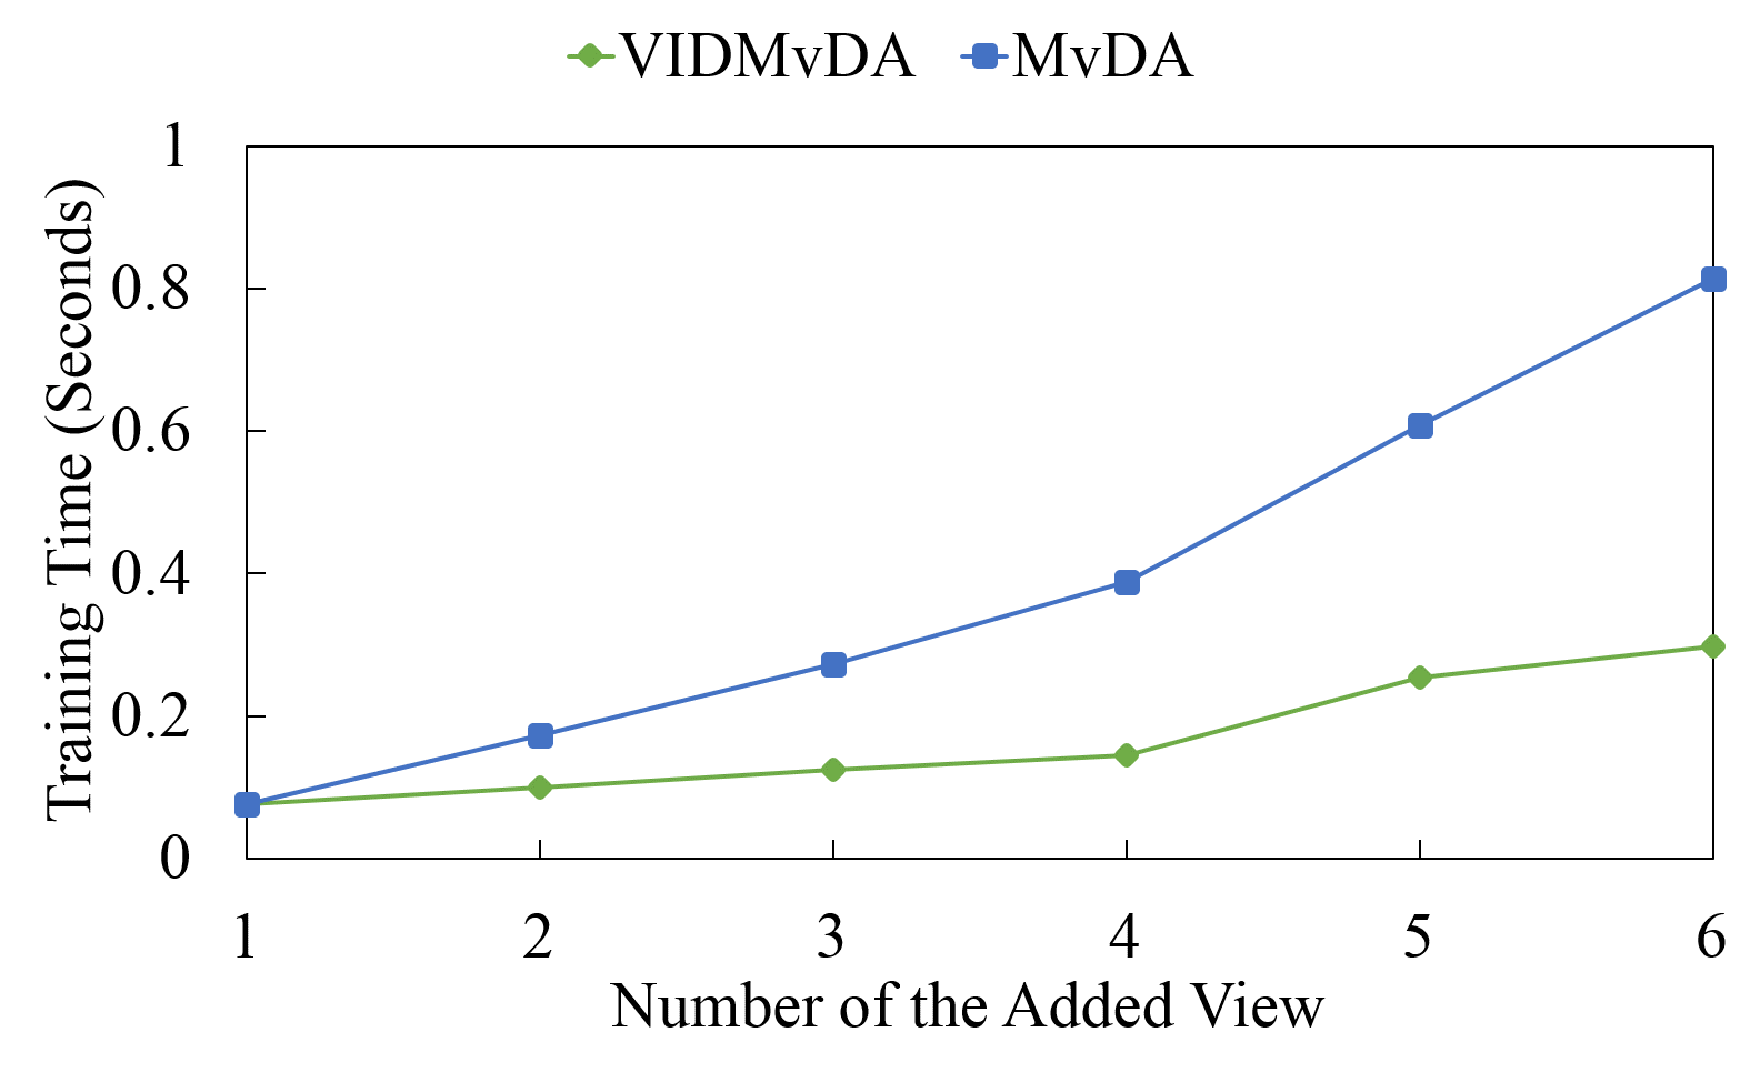
\includegraphics[width=\textwidth]{Figures/VIDMvDA/Fig6.pdf}
    \caption{Handwritten digits dataset}
    \label{fig:VIDMvDA_Res_Time_Add_Digits}
  \end{subfigure}
  \begin{subfigure}[h]{0.4\textwidth}
    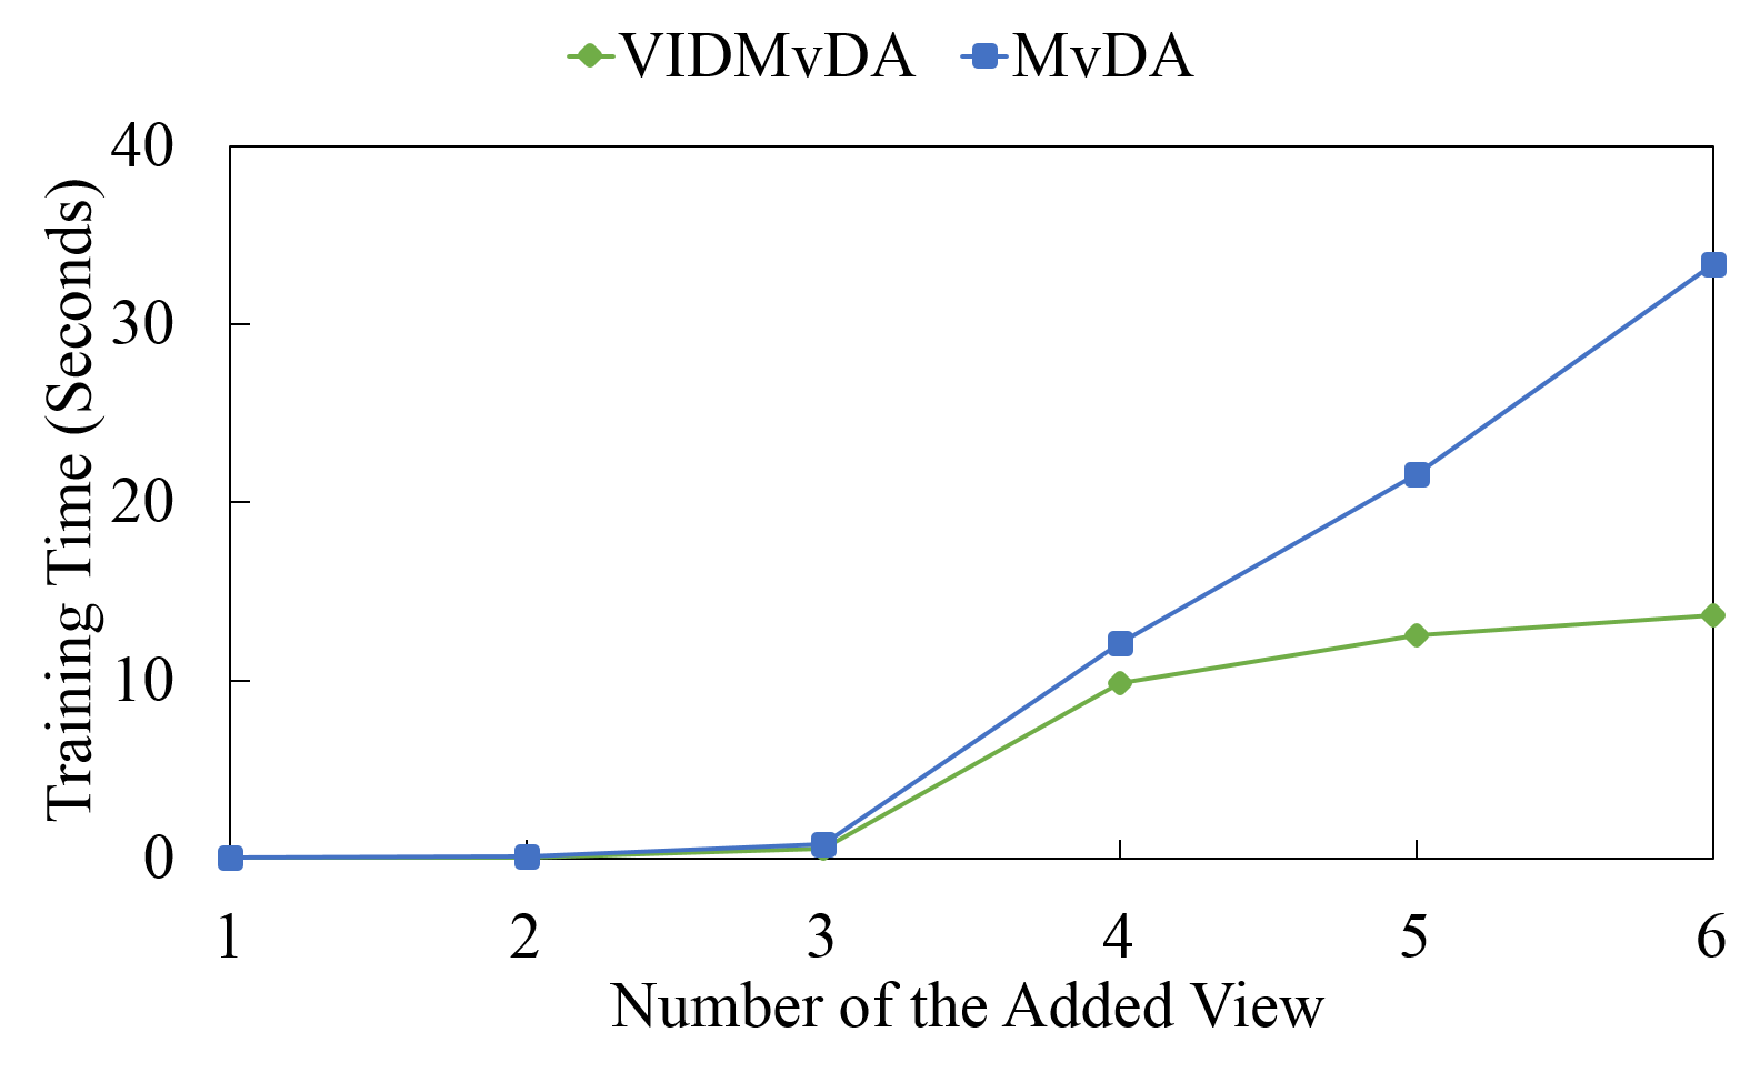
\includegraphics[width=\textwidth]{Figures/VIDMvDA/Fig7.pdf}
    \caption{Caltech-7 dataset}
    \label{fig:VIDMvDA_Res_Time_Add_Cal}
  \end{subfigure}
  
  \begin{subfigure}[h]{0.4\textwidth}
    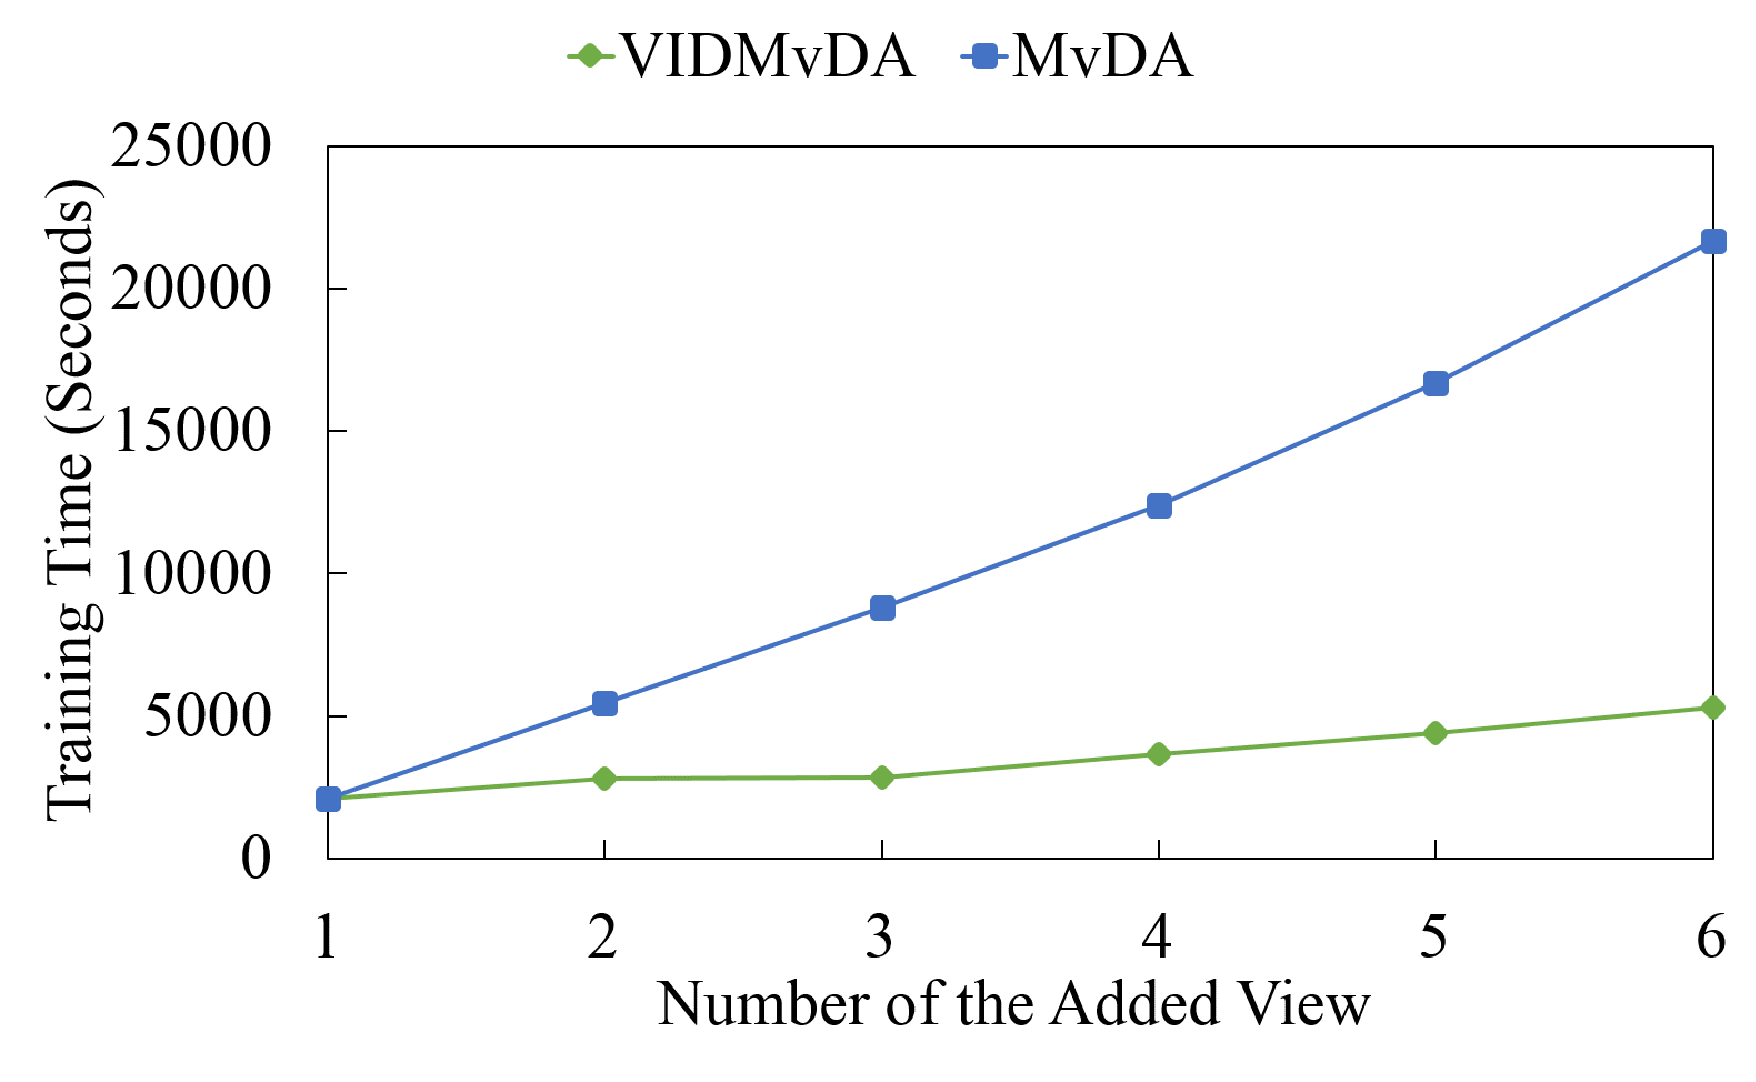
\includegraphics[width=\textwidth]{Figures/VIDMvDA/Fig8.pdf}
    \caption{AwA dataset}
    \label{fig:VIDMvDA_Res_Time_Add_AwA}
  \end{subfigure}
\caption{Addition of views : training time of VIDMvDA vs. MvDA}
\label{fig:VIDMvDA_Res_Time_Add}
\end{figure}

\begin{figure}
\centering
  \begin{subfigure}[h]{0.4\textwidth}
    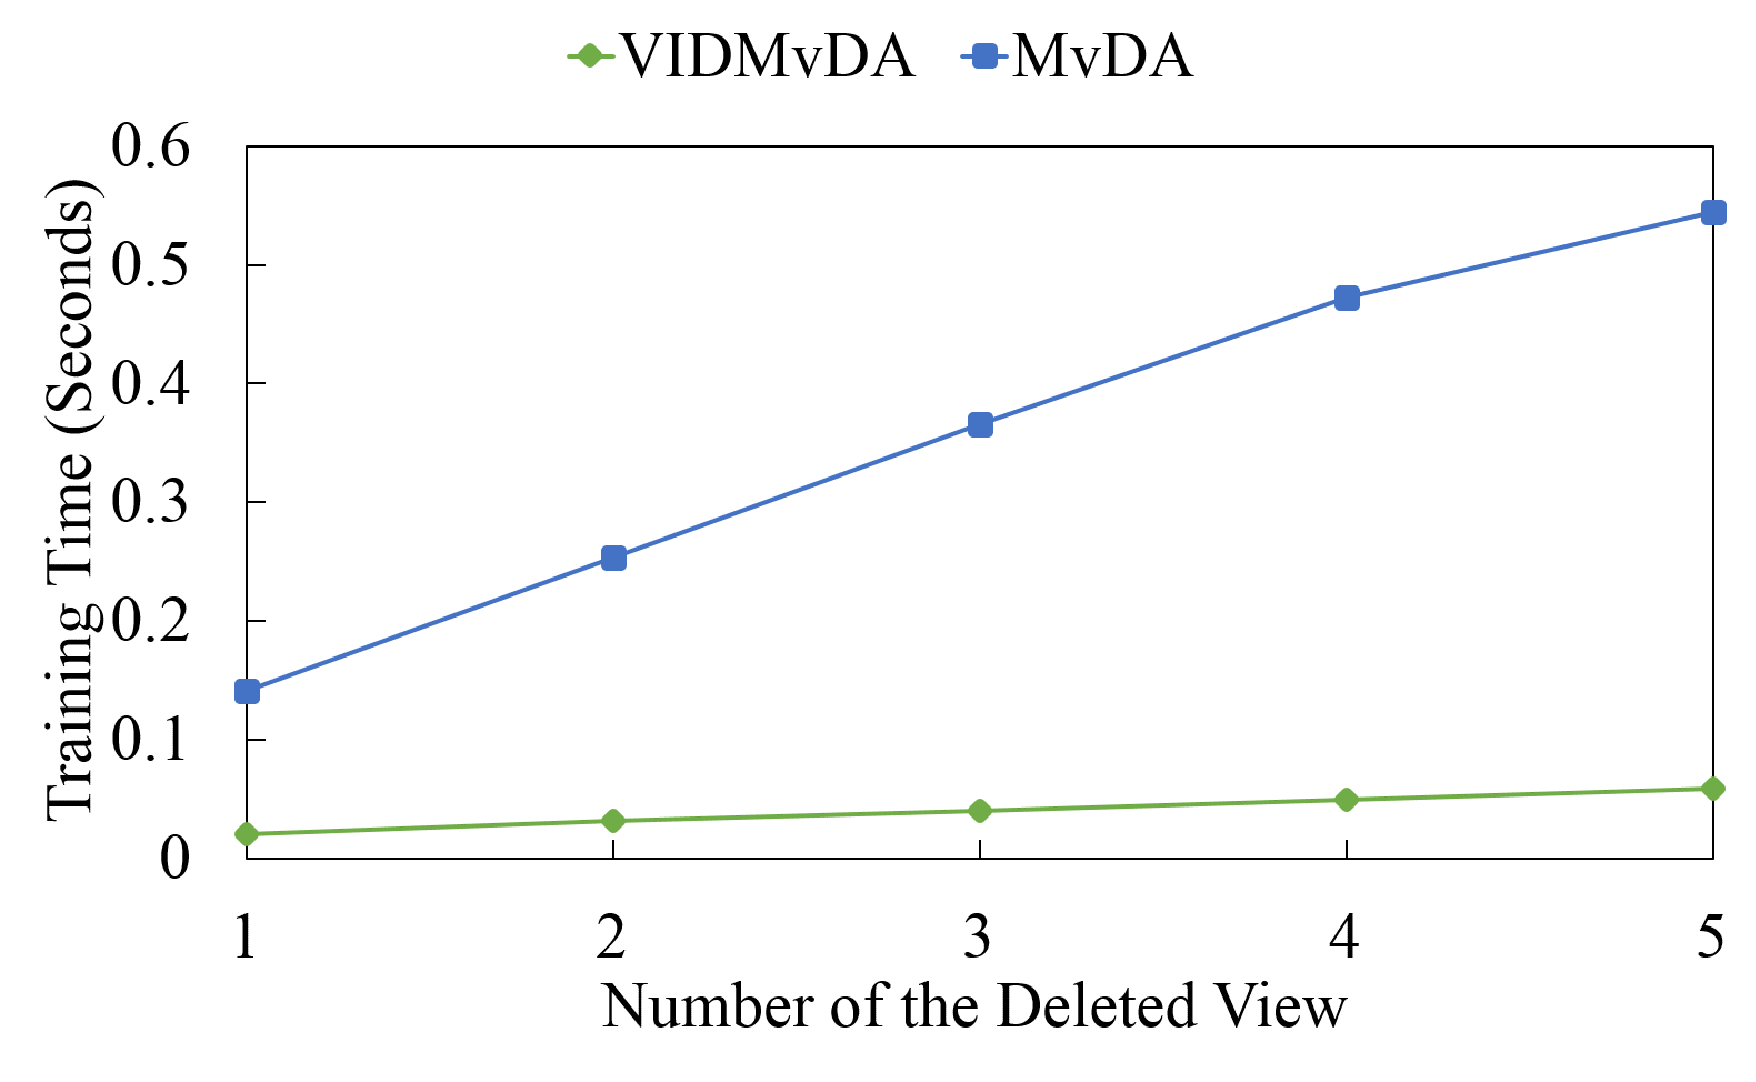
\includegraphics[width=\textwidth]{Figures/VIDMvDA/Fig9.pdf}
    \caption{Handwritten digits dataset}
    \label{fig:VIDMvDA_Res_Time_Del_Digits}
  \end{subfigure}
  \begin{subfigure}[h]{0.4\textwidth}
    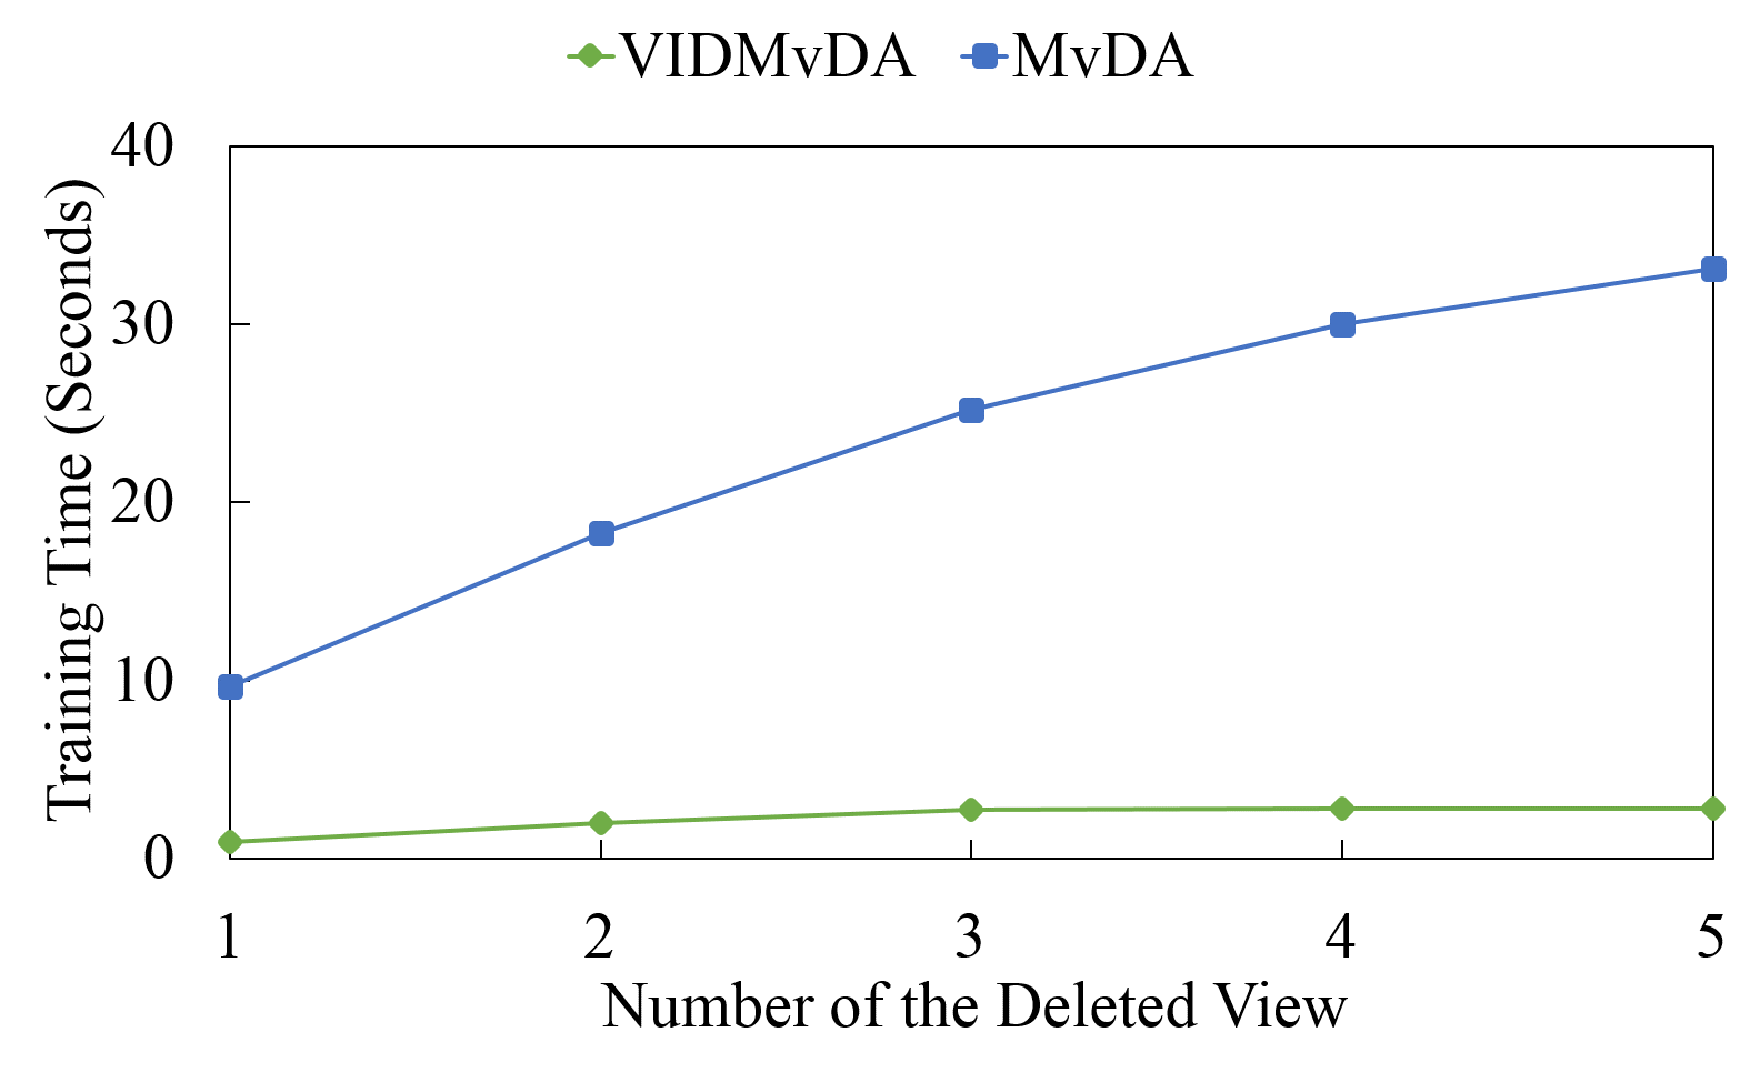
\includegraphics[width=\textwidth]{Figures/VIDMvDA/Fig10.pdf}
    \caption{Caltech-7 dataset}
    \label{fig:VIDMvDA_Res_Time_Del_Cal}
  \end{subfigure}
  
  \begin{subfigure}[h]{0.4\textwidth}
    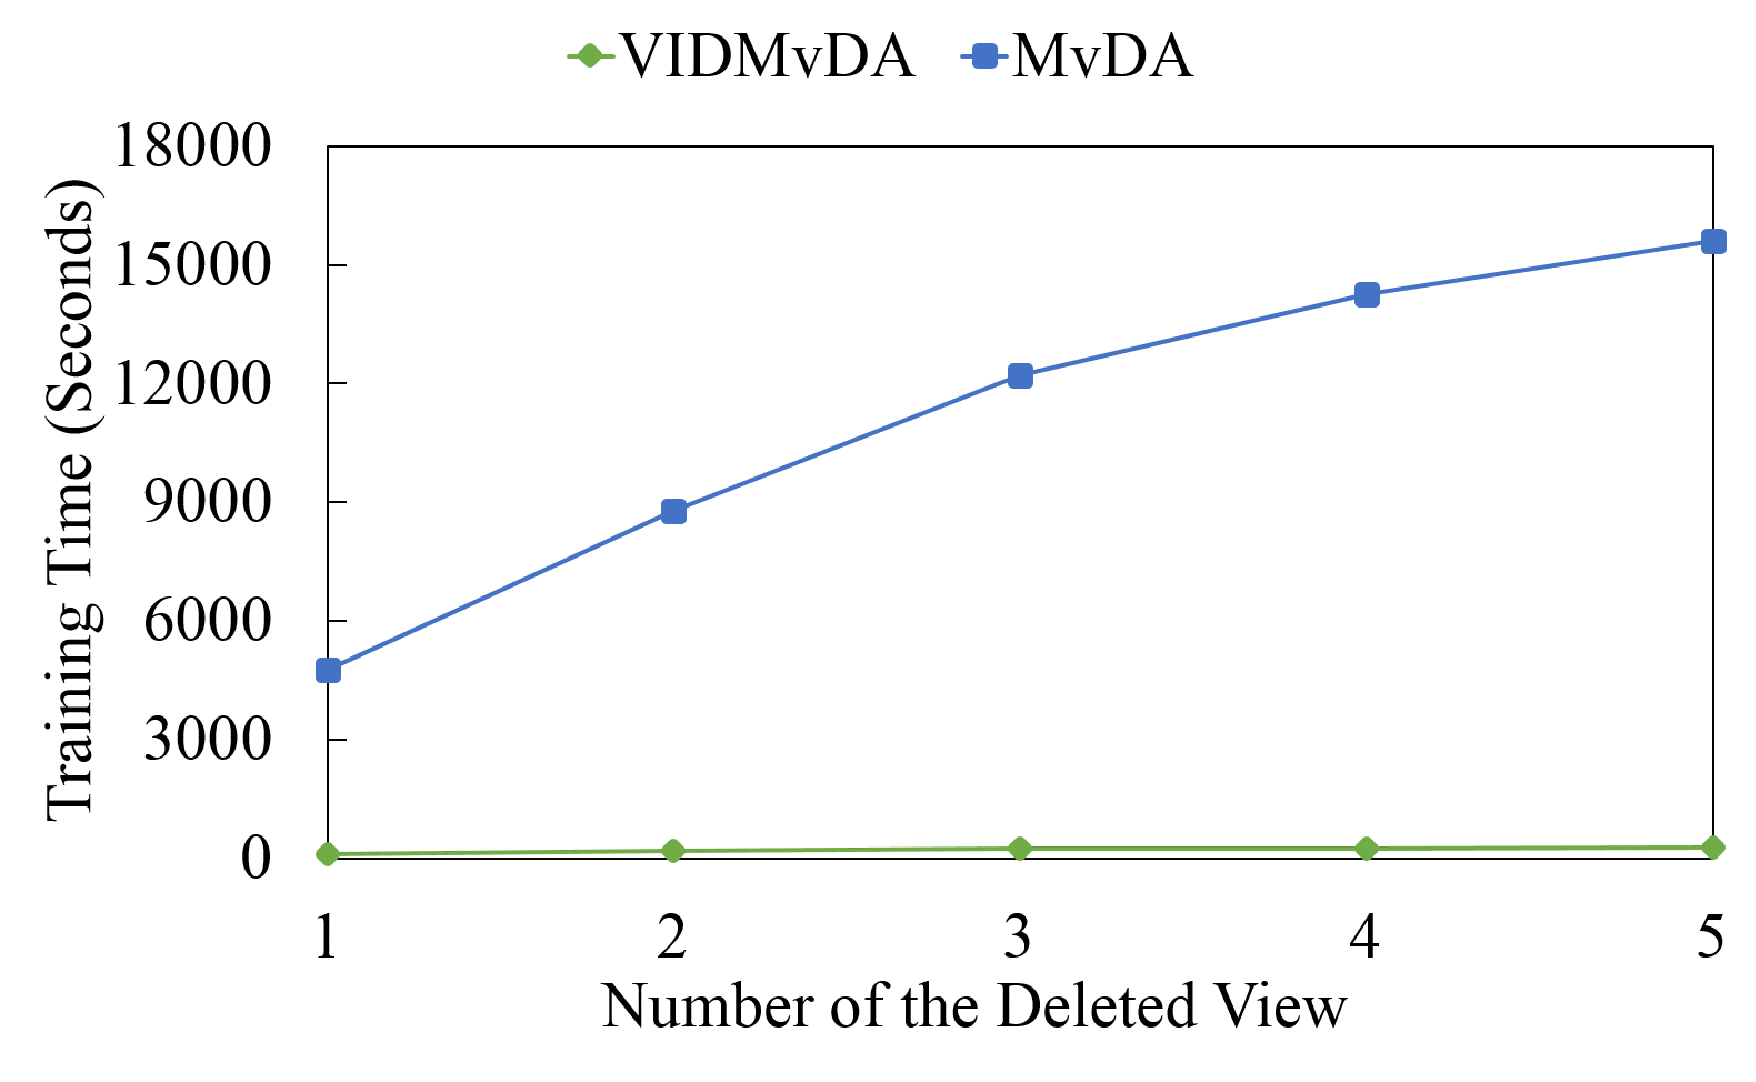
\includegraphics[width=\textwidth]{Figures/VIDMvDA/Fig11.pdf}
    \caption{AwA dataset}
    \label{fig:VIDMvDA_Res_Time_Del_AwA}
  \end{subfigure}
\caption{Deletion of views : training time of VIDMvDA vs. MvDA}
\label{fig:VIDMvDA_Res_Time_Del}
\end{figure}

\clearpage





%\begin{figure}[t]
%\centering
%  \begin{subfigure}[h]{0.4\textwidth}
%    \includegraphics[width=\textwidth]{Figures/VIDMvDA/Fig12.pdf}
%    \caption{Handwritten digits dataset}
%    \label{fig:VIDMvDA_Res_Time_Add_IM}
%  \end{subfigure}
%  \begin{subfigure}[h]{0.4\textwidth}
%    \includegraphics[width=\textwidth]{Figures/VIDMvDA/Fig13.pdf}
%    \caption{Caltech-7 dataset}
%    \label{fig:VIDMvDA_Res_Time_Add_MS}
%  \end{subfigure}
%  
%  \begin{subfigure}[h]{0.4\textwidth}
%    \includegraphics[width=\textwidth]{Figures/VIDMvDA/Fig14.pdf}
%    \caption{AwA dataset}
%    \label{fig:VIDMvDA_Res_Time_Add_SF}
%  \end{subfigure}
%  \begin{subfigure}[h]{0.4\textwidth}
%    \includegraphics[width=\textwidth]{Figures/VIDMvDA/Fig15.pdf}
%    \caption{AwA dataset}
%    \label{fig:VIDMvDA_Res_Time_Add_ORL}
%  \end{subfigure}
%\caption{Addition of views : training time of VIDMvDA vs. 2DMvDA}
%\label{fig:VIDMvDA_Res_Time_Add_2D}
%\end{figure}
%
%\begin{figure}
%\centering
%  \begin{subfigure}[h]{0.4\textwidth}
%    \includegraphics[width=\textwidth]{Figures/VIDMvDA/Fig16.pdf}
%    \caption{Handwritten digits dataset}
%    \label{fig:VIDMvDA_Res_Time_Del_IM}
%  \end{subfigure}
%  \begin{subfigure}[h]{0.4\textwidth}
%    \includegraphics[width=\textwidth]{Figures/VIDMvDA/Fig17.pdf}
%    \caption{Caltech-7 dataset}
%    \label{fig:VIDMvDA_Res_Time_Del_MS}
%  \end{subfigure}
%  
%  \begin{subfigure}[h]{0.4\textwidth}
%    \includegraphics[width=\textwidth]{Figures/VIDMvDA/Fig18.pdf}
%    \caption{AwA dataset}
%    \label{fig:VIDMvDA_Res_Time_Del_SF}
%  \end{subfigure}
%  \begin{subfigure}[h]{0.4\textwidth}
%    \includegraphics[width=\textwidth]{Figures/VIDMvDA/Fig19.pdf}
%    \caption{AwA dataset}
%    \label{fig:VIDMvDA_Res_Time_Del_ORL}
%  \end{subfigure}
%\caption{Deletion of views : training time of VIDMvDA vs. 2DMvDA}
%\label{fig:VIDMvDA_Res_Time_Del_2D}
%\end{figure}
%
%\clearpage













\subsubsection{Comparison of Memory Requirements}
\label{ssubs:VIDMvDA_Memory}
\begin{itemize}
\item \textbf{RQ5 :}
Can this method reduce memory requirements?

\item \textbf{Experiment :}
We record the total amount of storage taken by each model after training on all six views.

\item \textbf{Discussion :}
As VIDMvDA only stores the existing model and the new data samples instead of storing all the historical data along with the model, it requires less memory for training than the batch method. This is reflected in the recorded memory requirements. Table \ref{tab:VIDMvDA_Res_Mem} and Table \ref{tab:VIDMvDA_Res_Mem_2D} present the records of memory requirements of these methods on the 1D and 2D datasets, respectively.

We see that VIDMvDA requires much less memory than the batch methods. The difference between the memory requirements of these methods is again highlighted in the case of the AwA dataset. As it is a very large dataset, the required storage space is also significant. However, as VIDMvDA does not need to store all the historical data, it takes only 11 MBs, while MvDA takes around 7.5 GBs of memory.
\end{itemize}

\begin{table}[t]
	\centering
	\caption{Comparison of memory requirements (in MBs) of VIDMvDA and MvDA}
	\label{tab:VIDMvDA_Res_Mem}
	\begin{tabular}{l r r r} \toprule
		
		 & \textbf{Handwritten Digits} & \textbf{Caltech-7} & \textbf{AwA} \\ \midrule
		VIDMvDA &  0.34 \hspace{1.4cm} &   2.57 \hspace{0.3cm} & 11.07 \\ 
		MvDA    & 23.38 \hspace{1.4cm} & 292.55 \hspace{0.3cm} & 7535.07 \\ \bottomrule
	
	\end{tabular}
\end{table}


\begin{table}[t]
	\centering
	\caption{Comparison of memory requirements (in GBs) of VIDMvDA and 2DMvDA}
	\label{tab:VIDMvDA_Res_Mem_2D}
	\begin{tabular}{l c c c c} \toprule
		
		 & \textbf{IMPART} & \textbf{MSSpoof} & \textbf{Stereo Face} & \textbf{ORL} \\ \midrule
		VIDMvDA & 1.29 & 0.38 & 0.50 & 0.02 \\ 
		2DMvDA    & 5.44 & 7.61 & 3.94 & 0.18 \\ \bottomrule
	
	\end{tabular}
\end{table}









\section{Summary}
\label{sec:VIDMvDA_conc}
In this chapter, we have presented View Incremental Decremental Multi-view Discriminant Analysis (VIDMvDA), an incremental method for multi-view data that supports the addition and deletion of views over time. This method is based on discriminant analysis and provides closed-form solutions for incremental learning and decremental unlearning. In the case of increment, it produces the updated discriminant subspace using only the existing model and the newly added views. It also supports the deletion of any existing views and produces the updated subspace after the deletion using only the existing model. This provision allows it to train in much less time than the batch method. Also, as VIDMvDA does not need to store all the historical data, it requires much less memory than its batch counterpart, MvDA.

Through experiments, we have also shown that, while taking less time and memory, VIDMvDA constructs a similar discriminative subspace as MvDA. Hence, it also performs at par or sometimes better than MvDA in terms of classification accuracy. We have also proven that the order of addition or deletion of views does not affect the subspace construction of VIDMvDA.

%This work is submitted for peer-review to Applied Intelligence.

\chapterend
\cleardoublepage